%chapsimc.tex
%
\Section{General Overview}%
%
In order to take into account the multi-dimensional phase space of the experiment, this analysis required a Monte Carlo simulation of the experiment to extract the yield of $K^+$s which is used to extract the nuclear transparency. The simulation uses a model of the electro-production of kaons from protons which includes multiple scattering, energy loss from passage through materials, kaon decay, and correction due to radiative processes.

The simulation code used for this analysis was based upon the code SIMULATE used by the SLAC NE-18 experiment \cite{PhysRevC.64.054610}. The code has been modified to include magnetic transport models of the spectrometer, HMS and SOS of Hall-C in Jefferson Lab and has been renamed as SIMC.

%
\Section{Ingredients of SIMC}%
%
\label{Ingredients of SIMC}
In this section we give an overview of some of the basic ingredients of SIMC.
%SIMC is the Monte Carlo simulation for Hall-C which have some basic ingradients. We are trying to give an overview of few ingradients in this section.

\SubSection{Event Generation}
\label{Event Generation}
The event generator for electron-proton scattering consists of randomly generated energy-momentum 4-vectors for all the initial and final particles within the constraints of energy-momentum conservation in a two-body reaction (the kaon-hyperon production is a two-body process). The incident electron 4-vector is generated from the known beam energy, randomly smeared by the energy resolution (0.1\%). The target proton 4-vector just requires the proton mass since it is at rest. The outgoing particles 4-vectors are generated within the allowed acceptance of the spectrometers. The event generation also randomly picks an interaction point that is within the length of the target and consistent with the beam raster amplitude used in the experiment. With this complete set of information on the interaction vertex, we can calculate the physics variables $Q^2$, $W$, $t$ and $\phi_{pq}$. Here $Q^2$ is four-momentum transferred square, $W$ is the C.M. energy, $t$ is the momentum transfer and $\phi_{pq}$ is  the angle between the scattering and reaction planes. The event generation is performed for the selected species of hyperons Y = ($\Lambda^0$, $\Sigma^0$, $\Sigma^-$).

%The simulation starts with randomly generated 4-vectors for the outgoing kaon and electron. The 4-vectors for the target proton are needed to solve the kinematics. The event generator first randomly choose a target interaction point which is consistent with the target length and raster amplitudes in the beam coordinate system. The beam energy of a resolution 0.5\% is selected with the given value in the input file. Then different quantities like $Q^2$, w, t, $\phi_{pq}$ etc. are randomly generated for each event. The Monte Carlo input file also species which hyperon Y = ($\Lambda$, $\Sigma^0$) is being generated for the kaon side reaction. Kaon hyperon production is a two body reaction and the momentum of the outgoing kaon in the center of mass frame is fixed by knowledge of w. The quantities $Q^2$, w, t and $\phi_{pq}$ are defined in the Section \ref{Comparison of Data with SIMC}.

\SubSection{Spectrometer Simulation}
\label{Spectrometer Simulation}
SIMC has realistic models of the magnetic spectrometers including multiple scattering and energy loss in all intervening material encountered by the particles. All outgoing particles are transported through the magnets to the detector huts by a set of matrix elements that model the passage of charged particles through the magnetic elements of the spectrometer. The position and angle (track) information, smeared by the wire-chamber resolution, at the focal plane of the spectrometer are calculated for all particles that make it through the detector elements. The smeared track at the focal plane is then reconstructed back to the target using another set of matrix elements. This mimics the method used to analyze the data.
%elements which are sequential for both the SOS and HMS. The focal plane quantities can be calculated based on a smeared wire chamber positions when the particles make through the detector elements. The required detector elements for the SOS is Cerenkov aerogel plane. Particle are being reconstructed at the target by using focal plane quantities. More about reconstructed quantities are discussed in the Section \ref{Comparison of Data with SIMC}

\SubSection{Physics Model}
\label{Physics Model}
The kaon electro-production from a proton is depicted in \figureref{reaction1}. A model of this reaction is in the simulation, SIMC. The five fold-differential cross section for this process can be expressed in terms of a photoproduction cross section $\frac{d^2\sigma}{d\Omega_K^*}$ multiplied by a virtual photon flux factor $\Gamma(Q^2, W)$. 
%The electroproduction cross section can then be written in terms of the scattered electron energy $E^\prime$ , electron lab frame solid angle $d\Omega_e^\prime = dSin\theta_e d\phi_e$ and kaon C.M solid angle $d\Omega_K^* = dSin\theta_{qK}^* d\phi$. The form of the virtual photoproduction cross section used for this analysis is
\begin{equation} \label{equ:model1}
\frac{d^5\sigma}{dQ^2dWd\phi_{e}d\Omega^*_K} = \Gamma(Q^2,W) \left(\frac{d^2\sigma}{d\Omega^*_K}\right)
\end{equation}

In the simulation, a transformation between ($Q^2$,W) $\leftrightarrow$ ($E^\prime$,$\Omega_e^\prime$) is incorporated into the virtual photon flux, where $E^\prime$ is energy of the scattered electron and $\Omega^\prime_e$ is electron lab frame solid angle, using

\begin{equation} \label{equ:model2}
\Gamma(Q^2,W) =  \Gamma_0(E^\prime,\Omega^\prime_e) \frac{W}{2m_pEE^\prime} = \frac{\alpha}{4\pi^2}  \frac{(W^2-m^2_p)}{2m^2_pE^2} \frac{W}{Q^2} \frac{1}{(1-\epsilon)}
\end{equation}

%\begin{figure}[!tbp]
%  \centering
%  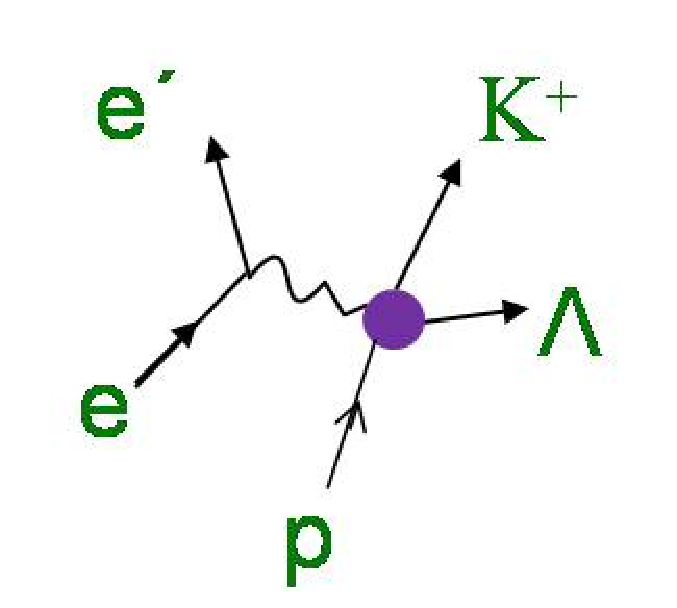
\includegraphics[width=0.4\columnwidth]{reaction1}
%  \caption[Schematic of kaon electro-production from proton.]{\label{fig:reaction1}Schematic of kaon electro-production from proton.}
%\end{figure}
\setlength{\figwidth}{0.4\linewidth}
\Figure{reaction1}{\figwidth}{Schematic of kaon electro-production from a proton.}
%In kaon transparency, the $K^+$ particle was detected in coincidence with the scattered electron, and therefore, the struck nucleon was constrained to be a proton by charge conservation. The struck proton was changed into a neutron by the interaction and a schematic of this process is shown in \figureref{reaction}.
\noindent
where $m_p$ is the mass of the proton and $\epsilon = \left(1 + \frac{2\left|\overline{q}\right|^2}{Q^2}\tan^2\frac{\theta_e}{2}\right)$ is the longitudinal polarization of the virtual photon.

The model for electro-production from nuclear targets schematically shown in \figureref{reaction2} was built from a parameterization of the measured cross section from a hydrogen target; for all other heavier targets (carbon, copper, gold) proton model is convoluted with a realistic spectral function for each target parametrized in terms of Eqs. \ref{equ:model1} and \ref{equ:model2}. Decay of kaons in flight and radiative corrections for all particles are also included in the model. 

\begin{figure}[!tbp]
  \centering
  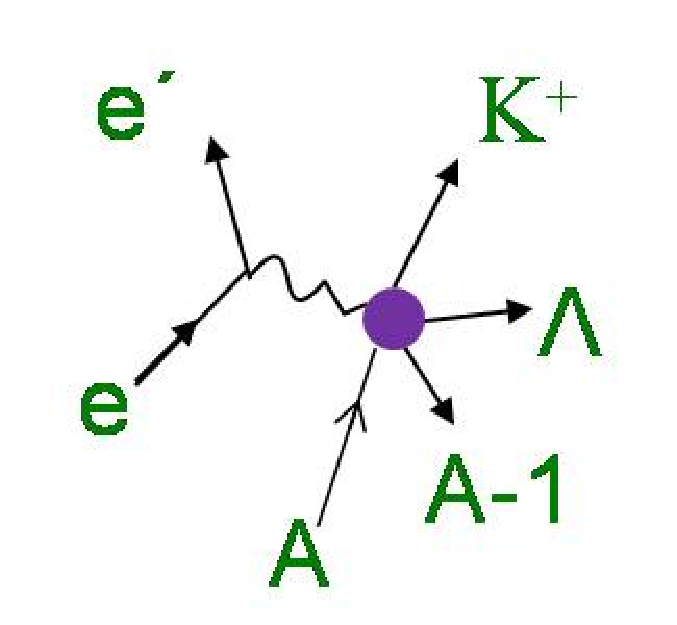
\includegraphics[width=0.4\columnwidth]{reaction2}
  \caption[Schematic of kaon electro-production from different targets.]{\label{fig:reaction2}Schematic of kaon electro-production from different targets.}
\end{figure}
%\setlength{\figwidth}{0.4\linewidth}
%\Figure{reaction2}{\figwidth}{Schematic of kaon electro-production from different targets.}

\SubSection{Kaon Decay}
\label{Kaon Decay}
In general, kaons are unstable and have a short mean lifetime which implies that a large fraction of the kaons which were created at the target decayed into secondary particles before they could be detected. The number of kaons that were actually detected was less than the true number of kaons produced in the reaction and corrections for their decay has been taken into account in the analysis ~\cite{RM99}. Kaon decay, multiple scattering, and energy loss are standard features in SIMC, and can be turned on and off using flags in the input files. Descriptions of corrections for these processes in the SIMC can be found in ~\cite{GaskelD}.

\SubSection{Spectral Function}
\label{Spectral Function}
The quasi-free model is used to describe electro-production from different nuclear targets used in the experiment. The incoming electron has larger energy compared to the binding energy of nucleons in the nucleus. So the bound nucleons in the target nucleus may be viewed as free nucleons. Properties of the nucleons inside of the nucleus are assumed to be described by an independent particle shell model, where each nucleon interacts with a mean field exerted by the other nucleons ~\cite{BC06}. The probability of finding a nucleon inside the nucleus with a certain energy and momentum can be defined by a spectral function. For heavier targets, the proton model is convoluted with a realistic spectral function for each target.

%
\Section{Comparison of Data with SIMC}%
%
\label{Comparison of Data with SIMC}
One of the goal of this analysis is to determine the normalized yields from the raw data collected during  the experiment. The normalized yield is the number of events that pass a given set of cuts divided by the cumulative charge delivered by the beam and corrected for the various inefficiencies of the experimental equipment. %Then transparency can be defined as the ratio of experimental yields from A $>$ 1 targets to hydrogen.
%
%\begin{equation} \label{equ:nucltransp1}
%T = 
%\frac{\bar Y_{\rm A}}{\bar Y_{\rm D}},
%\end{equation}
%
%$$T = \frac{Yield_A}{Yield_0}$$
%
%After comparing the data yields with SIMC yields, we have extracted nuclear transparency by forming a super ratio of the experimental yield to the Monte Carlo simulation yield, from nuclear targets and free protons (hydrogen), as shown in the expression below.
%
%\begin{equation} \label{equ:nucltransp3}
%T = 
%{\left( \frac{\bar Y}{\bar Y_{\rm MC}} \right)_A}/
%{\left( \frac{\bar Y}{\bar Y_{\rm MC}} \right)_{\rm D}},
%\end{equation}
%
%\begin{center}$$T=\frac{\frac{Yield_A^{data}}{Yield_A^{SIMC}}}{\frac{Yield_0^{data}}{Yield_0^{SIMC}}}$$\end{center}
%
%$\bar{Y}$ is the yield for data and $\bar{Y}_{MC}$ is for SIMC. A represent for the targets A$>$2 and D for Deuterium. The steps involved in extracting the normalized yields and transparency will be described in this chapter. Towards the goal of determining the nuclear transparency of kaons we have reconstructed the physical variables $Q^2$, W, t and $\phi_{pq}$ for each event at the interaction vertex. The measured yield is an integral over all of these variables.
%
%The cross section depends upon four variables, these are $Q^2$, W, t, $\phi_{pq}$. 

Before calculating the yields, we compare the data with SIMC yields, to verify that the Monte Carlo distributions agree with the measured distributions for these variables. If the shape of these distributions agree, it validates our model of kaon electro-production. The target quantities (horizontal slope $X_{tar}^\prime$, vertical slope $Y_{tar}^\prime$ and the momentum fraction of the particle with respect to the spectrometer central momentum $\delta$) were reconstructed using the focal plane quantities $X_{fp}$(horizontal position), $X_{fp}^\prime$ (horizontal angle), $Y_{fp}$ (vertical position) and $Y_{fp}^\prime$ (vertical position) on the focal plane\footnote{Focal plane is perpendicular to the central ray.} for HMS and SOS. The reconstructed angle and momentum fraction at the target are labeled as \textit{hsxptar}, \textit{hsyptar} and \textit{hsdelta} for the HMS and \textit{ssxptar}, \textit{ssyptar} and \textit{ssdelta} for the SOS.

%\setlength{\figwidth}{0.8\linewidth}
%\Figure{com_plot_Q2_2}{\figwidth}{$Q^2$. Clockwise from top left corener: $Q^2_\Lambda$ SIMC, $Q^2_\Sigma$ SIMC, $Q^2_\Sigma$ data, $Q^2_\Lambda$ data}

%\setlength{\figwidth}{1.0\linewidth}
%\Figure{Q2_2}{\figwidth}{$Q^2$ combined $\Lambda$ and $\Sigma$ for both SIMC and data}

%\setlength{\figwidth}{0.8\linewidth}
%\Figure{com_plot_w_2}{\figwidth}{W. Clockwise from top left corener: $W_\Lambda$ SIMC, $W_\Sigma$ SIMC, $W_\Sigma$ data, $W_\Lambda$ data}

%\setlength{\figwidth}{0.8\linewidth}
%\Figure{w_2}{\figwidth}{W combined $\Lambda$ and $\Sigma$ for both SIMC and data}

%\setlength{\figwidth}{0.8\linewidth}
%\Figure{com_plot_t_2}{\figwidth}{t. Clockwise from top left corener: $t_\Lambda$ SIMC, $t_\Sigma$ SIMC, $t_\Sigma$ data, $t_\Lambda$ data}

%\setlength{\figwidth}{0.8\linewidth}
%\Figure{t_2}{\figwidth}{t combined $\Lambda$ and $\Sigma$ for both SIMC and data}

%\setlength{\figwidth}{0.8\linewidth}
%\Figure{com_plot_phi_2}{\figwidth}{$\phi^{pq}$. Clockwise from top left corener: $\phi^{pq}_\Lambda$ SIMC, $\phi^{pq}_\Sigma$ SIMC, $\phi^{pq}_\Sigma$ data, $\phi^{pq}_\Lambda$ data}

%\setlength{\figwidth}{0.8\linewidth}
%\Figure{phipq_2}{\figwidth}{$\phi^{pq}$ combined $\Lambda$ and $\Sigma$ for both SIMC and data}

Beside applying cuts on $Q^2$, $W$, $t$ and $\phi_{pq}$, cuts were applied on these reconstructed quantities (such as \textit{hsxptar}, \textit{ssxptar}, \textit{hsyptar}, \textit{ssyptar}, \textit{hsdelta} and \textit{ssdelta}) both on the data and SIMC yields, as they define the feducial acceptance of the detector. In order to restrict the data to regions where they match the simulation, we applied very tight cuts on these fiducial acceptances. The cuts are discussed in Section~\ref{Cuts}.

%\setlength{\figwidth}{0.8\linewidth}
%\Figure{com_plot_2_ptar_2}{\figwidth}{Clockwise from top left corener: hsxptar, ssxptar, ssyptar and hsyptar. \textcolor{red}{RED} shows for SIMC and \textcolor{blue}{BLUE} shows for data}
%\setlength{\figwidth}{0.8\linewidth}
%\Figure{com_plot_sxptar_2}{\figwidth}{Clockwise from top left corener: $hsxptar_\Lambda$, $hsxptar_\Sigma$, $ssxptar_\Sigma$ and $ssxptar_\Lambda$. \textcolor{red}{RED} shows for SIMC and \textcolor{blue}{BLUE} shows for data}
\begin{figure}[!tbp]
  \centering
  \includegraphics[width=0.8\columnwidth]{com_plot_2_hms_2}
  \caption[HMS reconstructed angles and momentum fraction.]{\label{fig:com_plot_2_hms_2}HMS reconstructed angles and momentum fraction.\\\\ $hsxptar$, $hsyptar$, $hsytar$ and $hsdelta$ for $\Lambda$ production of $K^+$ after applying cuts on the variables. RED for SIMC and BLUE for data.}
\end{figure}
%\setlength{\figwidth}{0.8\linewidth}
%\Figure{com_plot_2_hms_2}{\figwidth}{HMS reconstructed angles and momentum fraction (hsxptar, hsyptar, hsytar and hsdelta) for $\Lambda$ production of $K^+$ after applying cuts on the variables. \textcolor{red}{RED} for SIMC and \textcolor{blue}{BLUE} for data.}

\begin{figure}[!tbp]
  \centering
  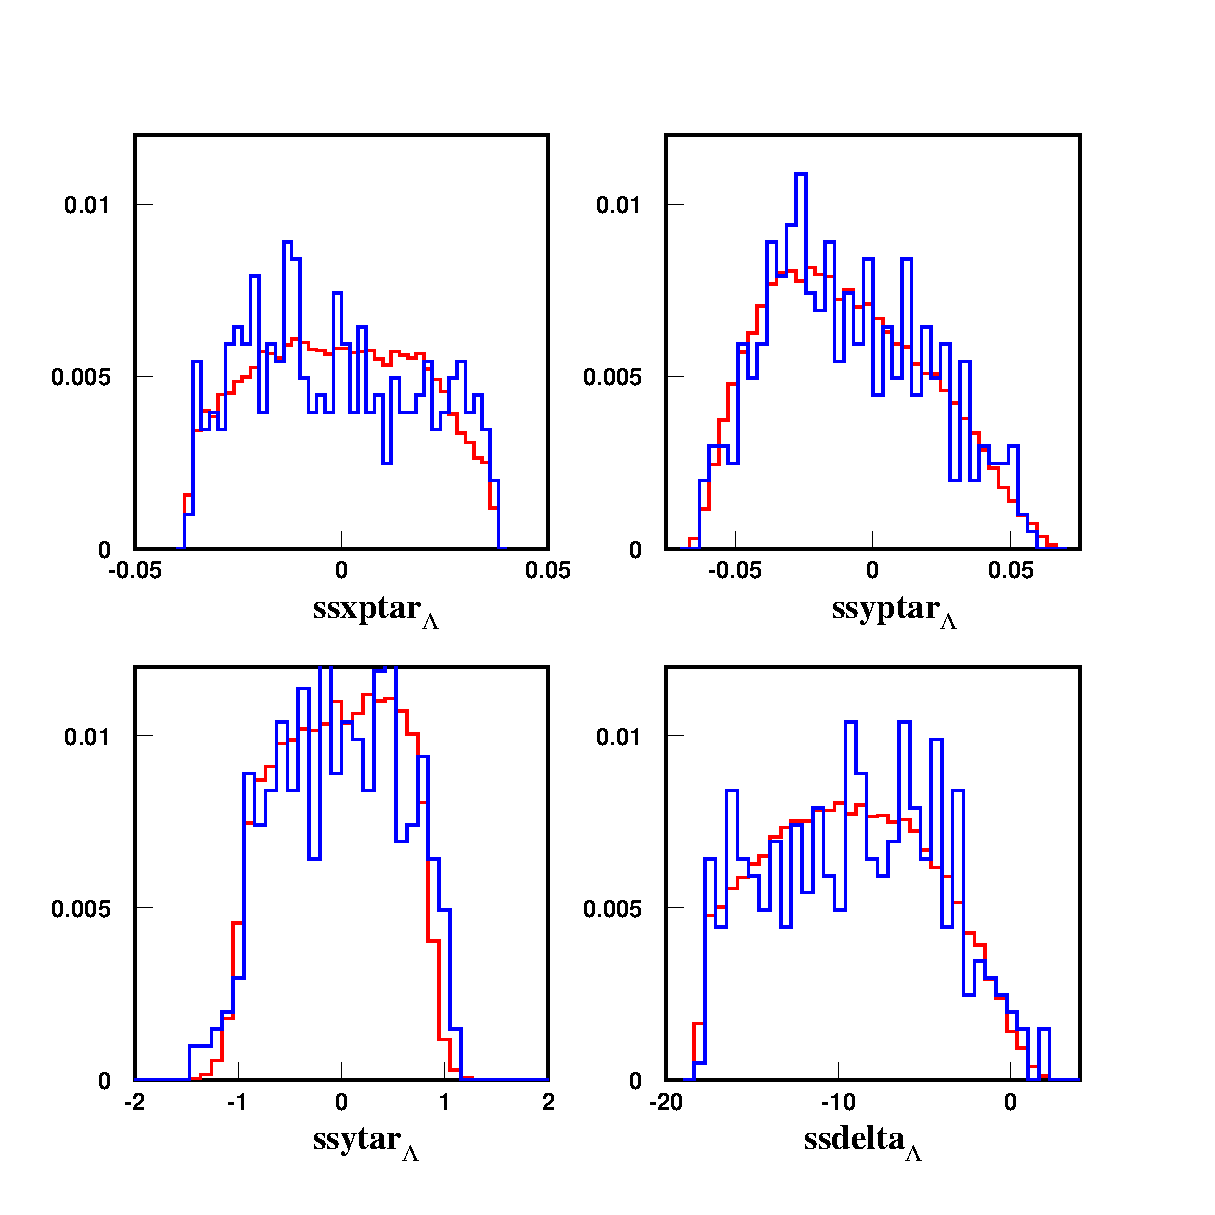
\includegraphics[width=0.8\columnwidth]{com_plot_2_sos_2}
  \caption[SOS reconstructed angles and momentum fraction.]{\label{fig:com_plot_2_sos_2}SOS reconstructed angles and momentum fraction.\\\\ $ssxptar$, $ssyptar$, $ssytar$ and $ssdelta$ for $\Lambda$ production of $K^+$ after applying cuts on the variables. RED for SIMC and BLUE for data.}
\end{figure}
%\setlength{\figwidth}{0.8\linewidth}
%\Figure{com_plot_2_sos_2}{\figwidth}{SOS reconstructed angles and momentum fraction (ssxptar, ssyptar, ssytar and ssdelta) for $\Lambda$ production of $K^+$ after applying cuts on the variables. \textcolor{red}{RED} for SIMC and \textcolor{blue}{BLUE} for data.}

As a representative sample, we have shown the comparison of data with SIMC yields for the reconstructed target variables in the case of $\Lambda$ production at $Q^2$ = 2.2 $\mathrm{(GeV/c)^2}$. BLUE and RED show data and SIMC, respectively, for the HMS in \figureref{com_plot_2_hms_2} and for the SOS in \figureref{com_plot_2_sos_2}. Similarly comparisons were also performed for $\Lambda$ and $\Sigma$ production at $Q^2$ = 1.1 to 3.0 $\mathrm{(GeV/c)^2}$, but are not shown here.

%Cuts on these feducial acceptances are being shown in the \figureref{com_plot_2_hms_2} and \figureref{com_plot_2_sos_2}. We have compared data with SIMC for the reconstructed target variables in case of $\Lambda$ production of kinematics $Q^2$ = 2.2 $(GeV/c)^2$ shown by \textcolor{blue}{BLUE} and \textcolor{red}{RED} respectively for HMS in the \figureref{com_plot_2_hms_2}. Same has been shown for SOS in the \figureref{com_plot_2_sos_2}. Similarly we applied for $\Sigma$ production for this kinematics and considered other kinematics of $Q^2$ = 1.1, 3.0 $(GeV/c)^2$ as well.